\section{Giới thiệu}
\subsection{Giới thiệu mô hình}
Mô hình được sử dụng trong bài thực hành là \textbf{YOLOv10}, đây là phiên bản \textbf{YOLO} được phát hình vào tháng 5/2024. Lí do sử dụng mô hình \textbf{YOLOv10} thay cho \textbf{YOLOv4} là do sự tương thích của \textbf{YOLOv10} với phiên bản hiện tại của Colab là 3.10.12 (so với \textbf{YOLOv4} là 3.6/3.7). Đồng thời tránh việc xung đột giữa các thư viện được yêu cầu cài đặt so với các thư viện hiện có trong Colab.

\subsection{Đánh giá hiệu suất mô hình}

\begin{figure}[H]
    \centering
    \subfigure[ ]{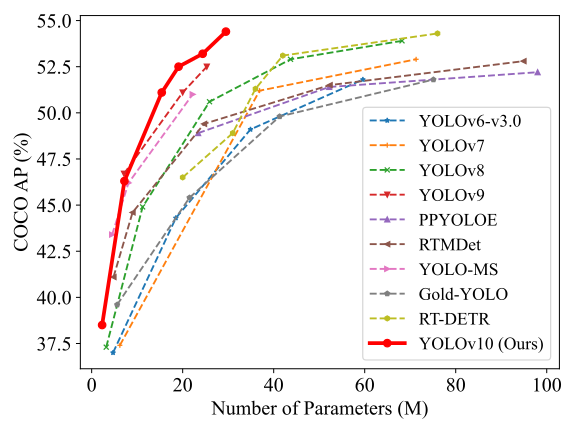
\includegraphics[scale=0.4]{img/params.png}}
    \quad % Khoảng cách ngang giữa các ảnh
    \subfigure[ ]{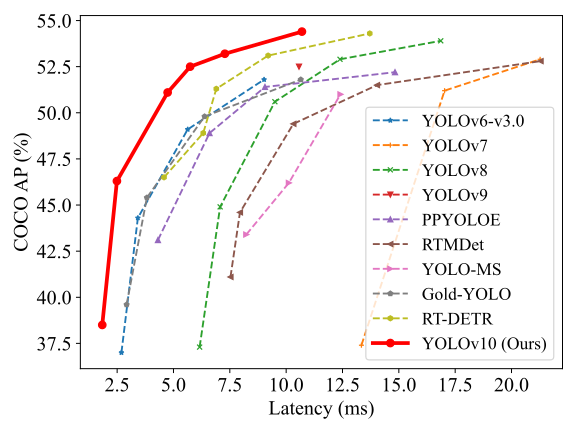
\includegraphics[scale=0.4]{img/latency.png}}
    \caption{Đánh giá hiệu suất các mô hình theo độ trễ (Latency) và số tham số (Parameters)}
    \label{fig:multiple_images}
\end{figure}

Các mô hình được đánh giá trên tập dữ liệu COCO. Về số lượng tham số, YOLOv10 cho thấy độ chính xác cao nhất ở mức tham số nhỏ và vừa. Đồng thời ở giá trị độ trễ, YOLOv10 cũng cho độ chính xác tốt nhất ở các mức độ trễ thấp nhất. Điều này cho thấy YOLOv10 đã cải thiện đáng kể về cả độ chính xác, hiệu năng và tốc độ xử lí so với các mô hình tiền nhiệm. 